\section{Inter-GPU communication without CPU Intervention}
In this section, we talk about GPUDirect technology for communicating between GPUs without any CPU intervention via Remote Dynamic Memory Access (RDMA). Then we talk about our attempt to implement the GPUDirect technology in the Gluon communication substrate.
We further discuss about the challenges that we faced in this implementation and conclude this section with our insights. 

\subsection{GPUDirect Technology}
Message Passing Interface (MPI) is a standard API for data communication using messages among distributed processes
and commonly used in High Performance Computing (HPC).
The MPI standard defines various message-passing techniques which covers from point-to-point messages to collective operations like broadcastings. 

\begin{figure}
\centering
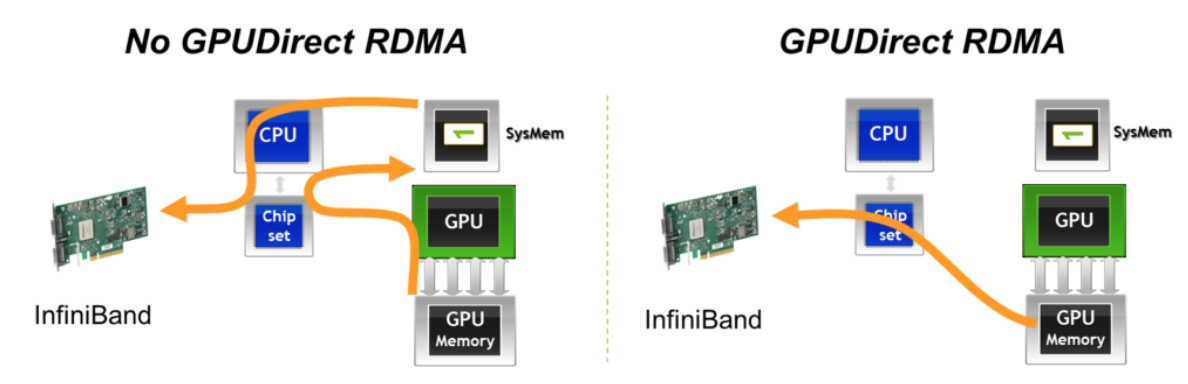
\includegraphics[width=0.49\textwidth]{gpu-rdma.png}
\mycaption{GPUDirect RDMA}{The figure shows the data transfers with and without GPUDirect RDMA. 
}
\label{fig-rdma}
%\vspace{-20pt}
\end{figure}

\begin{figure}
\centering
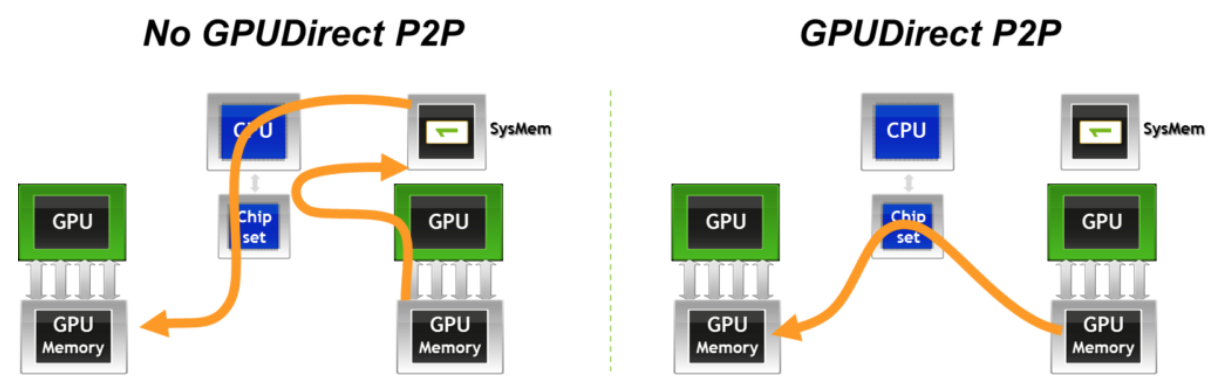
\includegraphics[width=0.49\textwidth]{gpu-ptp.png}
\mycaption{GPUDirect Peer-to-Peer}{The figure shows the data transfers with and without GPUDirect Peer-to-Peer. 
}
\label{fig-ptp}
%\vspace{-20pt}
\end{figure}


NVIDIA GPUDirect technologies provide high-bandwidth, low-latency communications with NVIDIA GPUs.
Remote Direct Memory Access (RDMA) is one of the newest GPUDirect technology which allows GPUs to
send its data directly to a network adapter without host memory participation. This is shown in Figure~\ref{fig-rdma}.
Another variant of this is Peer-to-Peer (P2P) transfers, which can accelerate intra-node communication.
Buffers can be directly copied between the memory of multiple GPUs in the same system through GPUDirect P2P. This is shown in Figure~\ref{fig-ptp}. 
Note that GPUDirectRDMA should exploit UVA technology; Otherwise, RDMA does not work since the MPI API calls on the host side cannot
recognize and point to GPU address.
GPUDirect technology also can be combined with other recent technologies such as asynchronous data transfer.

\subsection{GPUDirect in Gluon}
We attempted to implement the GPUDirect P2P and GPUDirect RDMA transfers on the Gluon Substrate
to accomplish direct inter-GPU communications without the host.
To support this functionality, we only aim for round based bfs\_push of lonestardist.
Gluon code is enormous and only for the one application, we had to modify entire execution paths of Gluon substrate.
The following lists show inter-GPU communication stages of the original Gluon.
\begin{enumerate}
\item Offsets and bitsets of the updated nodes are computed at the source GPU.
\item The computed data including the updated node label data are gathered, copied and serialized into a newly allocated CPU buffer.
\item The CPU buffer is transferred through asynchronous MPI APIs.
\item The sent CPU buffer is received at the destination CPU through asynchronous MPI APIs.
\item The received CPU buffer is deserialized and copied to the destination GPU.
\end{enumerate}
Using the GPUDirect Technology in this workflow, we can greatly reduce the overheads in these transfers, to the following steps:
\begin{enumerate}
\item Offsets and bitsets of the updated nodes are computed at the source GPU.
\item The computed date including the updated node label data are gathered, serialized and transferred directly from the source GPU using cuda-aware asynchronous MPI APIs supported by GPUDirect RDMA.
\item The sent data is directly received at the destination GPU using synchronous MPI.
\item The received data is deserialized and scattered to the proper locations. All of them are done on GPU.
\end{enumerate}
Note that all the steps can occur simultaneously along with other CPU computations. 
To do this, we also additionally apply asynchronous cuda memory copy with multiple streams, which avoids CPU blocking.
This feature, if applied effectively, has the potential to significantly improve the performance of data transfers, as compared to the other two features.

\subsection{Discussion and Limitations}
In this section, we introduce more detailed information about implementation.
The biggest challenge on this project was the current flow of MPI communications.
The following lists show how the current Gluon processes MPI messages. 
\begin{enumerate}
\item When Gluon substrate is initialized, the background thread called worker thread starts to run in background.
Until BFS finishes, the thread polls and catches all the OpenMPI messages received on the node.
\item All MPI message processings are done asynchronously.
If any message processing is done, then it moves to either receive vector or send vector.
Each vector comprises to buffer lists indexed by the host id. For example, the first item of the receive vector
contains buffer lists sent by the host 1.
\item For each round of BFS, the Gluon substrate enumerates the receive vector and checks whether any host sends 
message and the message is fully received ot not.
If it is, the substrate starts to process the received buffer. 
\end{enumerate}

All the above sequences are performed on \textit{CPU}.
However, GPUDirect messages should be received by GPU, not CPU.
To do this, GPU buffers should be preallocated before message receives with proper size, and 
gathered by the worker thread.
In addition, we need a GPU vector type to store and handle send and receive messages invoked dynamically. 
We can reuse the current Gluon network system in the future, but for this project, 
we just focused on the basic GPUDirect RDMA supports.
First, we use one fixed tag, 10000, for OpenMPI GPUDirect messages and make the worker thread ignore them.
Second, we remove the original serialization/deserialization/copy/scatter codes for CPU-GPU communications and 
replace them to GPU-GPU gather and scatter communications. In this case, we also serialize and deserialize 
message in order to avoid complex network system. But it is done only on GPU, not CPU.
Finally, the main thread requests MPI send or receive the serialized buffer messages, not the worker thread.

Our current implementation is the first attempts to support GPUDirect techniques on Gluon.
Therefore, it has several limitations, but also implies that there are lots of rooms for improvements.
First, since we could not collect GPU data to be sent or to be received, due to the shortage of 
stable GPU vector type, we only aimed for one-to-one GPU communication.
Therefore, in the future, we could improve and extend the current communication between two GPUs to multiple GPUs communication.
Second, we use asynchronous MPI send and synchronous MPI receive.
Using asynchronous MPI receive would improve performance.
This is also doable after we make GPU vector. As the original Gluon network does, 
asynchronous messaging would be processed in the background.
Third, GPUDirect RDMA can easily apply future optimizations of other techniques such as locality-aware memory management,
memory reuse and pinned memory.
